\documentclass[conference]{IEEEtran}
\IEEEoverridecommandlockouts
% The preceding line is only needed to identify funding in the first footnote. If that is unneeded, please comment it out.
%\usepackage{cite}
\usepackage{amsmath,amssymb,amsfonts}
\usepackage{algorithmic}
\usepackage{graphicx}
\usepackage{textcomp}
\usepackage{xcolor}

%\usepackage{aa228-jmlr2e}
\usepackage{lipsum}
\usepackage{listings}
\usepackage{color}
\usepackage{hyperref}
\hypersetup{%
	colorlinks=true,
	linkcolor=blue,
	linkbordercolor={0 0 1}
}

\lstset{ % General setup for the package
	language=python,
	basicstyle=\footnotesize\sffamily,
	numbers=left,
	numberstyle=\small,
%	frame=tb,
	tabsize=4,
	columns=fixed,
	showstringspaces=false,
	showtabs=false,
	keepspaces,
	commentstyle=\color{blue},
	keywordstyle=\color{purple},
	emph={function, elseif, end, true, false},
	emphstyle=\color{purple},
}
%\def\BibTeX{{\rm B\kern-.05em{\sc i\kern-.025em b}\kern-.08em
 %   T\kern-.1667em\lower.7ex\hbox{E}\kern-.125emX}}

\usepackage[square,numbers]{natbib}
\bibliographystyle{abbrvnat}

% \bibliographystyle{ieeetran}

 
\begin{document}

\title{Autonomous Driving in a Roundabout With Rule-Breaking Agents}

\author{\IEEEauthorblockN{Emiko Soroka}
\IEEEauthorblockA{\textit{AA 228 Final Project, Department of Aeronautics \& Astronautics} \\
\textit{Stanford University}\\
esoroka@stanford.edu}
%\and
%\IEEEauthorblockN{2\textsuperscript{nd} Given Name Surname}
%\IEEEauthorblockA{\textit{dept. name of organization (of Aff.)} \\
%\textit{name of organization (of Aff.)}\\
%City, Country \\
%email address or ORCID}
}

\maketitle

\begin{abstract}
While intersection are often used as a test case for interaction in autonomous driving, a roundabout is another interesting case where multiple agents interact. In this paper we design a discrete MDP to represent traversing a roundabout with other agents, learn the optimal policy for navigating a roundabout, and investigate how the policy changes when some agents break the rules of the road.
\end{abstract}

%\begin{IEEEkeywords}
%\end{IEEEkeywords}

\section{Introduction}
Roundabouts are relatively uncommon compared to intersections in the US,
but are rising in popularity due to their safety and environmental benefits \cite{MANDAVILLI2008135}. Studies have found that replacing signalized intersections with roundabouts improves throughput for low-speed intersections and reduces the risk of rear-end collisions \cite{persaud2001safety, saccomanno2008comparing}. One empirical study conducted in the US found that replacing intersections with roundabouts effected a 40\% reduction in crashes, with an even greater decrease in traffic injuries and deaths \cite{persaud2001safety}.

Although roundabouts are simple to navigate, with the cardinal rule being that traffic entering the roundabout yields to traffic already in the circle, human drivers who are unaware of this rule often hold up traffic by stopping in the roundabout. We are interested in two questions:
\begin{itemize}
	\item Can we train a reinforcement learning (RL) agent to successfully navigate a roundabout?
	\item How do rule-breaking drivers affect the optimal policy for navigating the roundabout?
\end{itemize}

\section*{Problem Description}
We represent this problem as a Markov decision process (MDP) over discrete states and actions. Although many papers have focused on RL in large problem spaces and complex models for autonomous driving \cite{kiran2021deep, zhu2020safe}, we will reduce the implementation difficulty by defining a small, discrete problem space.

\subsection{States} We define three integer-valued states: $s_1$, $s_2$ and $s_3$ (Fig. \ref{fig:statespace}).
\begin{itemize}
	\item
$s_1$ has 30 values, corresponding to the rounded distance traveled along the lane.
 \item
$s_2$ is the distance between the ego vehicle and the closest vehicle that presents a collision risk (see \ref{subs:collision}). This distance ranges from $0$ to $10$.
\item
$s_3$ is the ego vehicle velocity, sorted into buckets from $0$ to $10$.
\end{itemize}

\begin{figure}[h!]
	\centering
	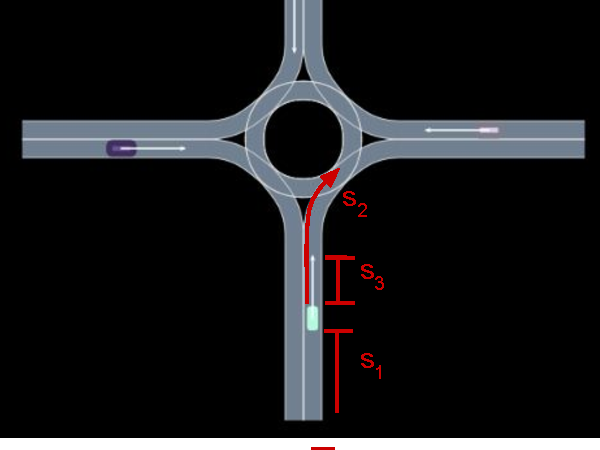
\includegraphics[width=0.8\linewidth]{figures/statespace.pdf}
	\caption{The three discretized state space variables.}
	\label{fig:statespace}
\end{figure}

\subsection{Actions} Our RL agent has three actions available: \verb|ZERO| (no acceleration action), \verb|ACCEL| and \verb|DECEL|. Lane-keeping is managed separately to simplify the problem, and no lane changes take place.

With this representation, there are $|S_1|\times|S_2|\times|S_3| = 3630$ states and 3 actions. This is a relatively small problem, so it is possible to learn an optimal policy by a direct method such as Bellman iteration.

\subsection{Observations} We assume there is no noise in the system and the states are directly observed.

\subsection{Reward} The RL agent receives a time-based reward $R(t)$ (Eq. \eqref{eq:reward}) for reaching its goal on the other side of the roundabout, where $N$ is the number of time steps in the simulation and $t$ is the step where the goal is reached. This incentivizes crossing the roundabout quickly. If a collision occurs, the agent receives a reward of $-1000$ and the simulation stops.

\begin{equation}
R(t) = \begin{cases}
10 + (N-t) & \text{ for reaching the end at step }t
\\
0.1\Delta s & \text{ for traveling $\Delta s$ in $N$ steps}
\\
-1000 & \text{ for collisions.}
\end{cases}
\label{eq:reward}
\end{equation}

\section{Modeling Other Drivers}
To provide other agents for the simulation, we defined two fixed policies by observing human drivers at the Manzanita Field roundabout.
\subsection{Rule-Following Driver Model} The rule-following driver model approximates the correct way to navigate a roundabout. When approaching, it yields to traffic already in the roundabout. If another vehicle is too close, it decelerates unless said vehicle is not currently in the roundabout. Otherwise, it prefers to maintain a constant speed.

This model can be represented by the code:
\begin{lstlisting}[language=python,caption={Rule-following driver model.}]
function get_lawful_action(model)
    # If distance to another car is < 2
    # and we are NOT in the roundabout
    if model.s2 < 2 &&
       (model.s1 < L || model.s1 > 2*L)
        return :DECEL
    # maintain speed
    elseif model.s3 >= 10
        return :ZERO
    # speed up to desired speed
    else
        return :ACCEL
    end
end
\end{lstlisting}

\subsection{Rule-Breaking Driver Model}
The rule-breaking driver behaves like the rule-following driver with probability $p \in [0,1]$. With probability $1-p$ it may take a rule-breaking action such as:
\begin{itemize}
	\item Yielding to a vehicle waiting to enter the roundabout.
	\item Not yielding to another vehicle when entering the roundabout.
\end{itemize}
This model can be represented by the code:
\begin{lstlisting}[language=python,caption={Rule-breaking driver model.}]
function get_lawless_action(model)
    # Should we yield when entering??
    if rand() < model.p && model.s2 < 2 &&
      (model.s1 == 1 || model.s1 == 3)
        return :DECEL
    # Should we stop in the roundabout??
    elseif rand() > model.p && model.s2 < 2
        returj :DECEL
    # stay at desired speed
    elseif model.s3 >= 10
        return :ZERO
    # speed up if too slow
    else
        return :ACCEL
    end
end
\end{lstlisting}

\textbf{Note:} As becomes clear later, these two agents are not particularly skilled at navigating the intersection.
\begin{figure}[h!]
	\centering
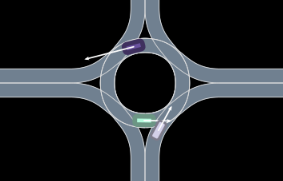
\includegraphics[width=0.7\linewidth]{figures/unsafe.png}
\caption{The unsafe driver (gray) enters the roundabout in front of the rule-following green car, causing a collision.}
\label{fig:unsafe}
\end{figure}

\section{Methodology}
We used \verb|AutomotiveSimulator.jl| \cite{simulator.jl} to define the environment, rule-breaking and rule-following agents, and the RL agent itself.
We used online Bellman iteration \cite{kochenderfer2022algorithmsch7} to learn the roundabout policy by running the simulation with varying starting positions and other agents.
We studied two cases.

\textbf{All rule-following drivers:} The other drivers yield correctly. Since Bellman iteration is exact, we expect this to converge to an optimal policy for navigating the roundabout.

\textbf{Some rule-breaking drivers:} A fraction $r\in (0,1)$ of the drivers break the rules with probability $p$. We used $p=0.5$, $r=0.25$ and $r=0.5$.

\subsection{Exploration:} We initially tested several different methods of balancing exploration vs exploitation and settled on a constant 50\% chance of taking a random action during training. Other approaches tested included:
\begin{itemize}
	\item Greedy selection: this did not work because the agent did not explore enough of the state space and never learned to move forward.
	\item Decreasing the exploration over time: this turned out to be unnecessary.
\end{itemize}

\section{Implementation} Most of the work on this project was in coming up with a reasonable discretization of the state space and debugging issues related to reward and simulation design.

\subsection{State Space and Reward} The space was chosen to be large enough to capture the desired behavior while still being tractable. Various modifications had to be made to resolve problems.
For example, we initially tried to use three states to capture position: before, in, and after the roundabout. This failed because the RL agent would take an action and remain in the same state, so it wasn't able to train.

We also tested several reward functions before settling on an appropriate one - some tests only gave a positive reward for crossing the roundabout, but the agent wasn't able to reach it before the simulation ended and again, didn't train effectively.

\subsection{Simulation Design} A final major issue was preparing simulations that effectively explored the state space. Initial simulations used three other agents, randomly assigned to each lane, but this resulted in very few observed states where a collision was possible. The resulting agent was unlikely to decelerate and avoid collisions. We increased this number to 5, ensuring that the agent encounters situations with and without another car sharing its lane.

\subsection{Collision Course Detection}\label{subs:collision}
A major challenge was defining and fine-tuning the human driver models for the RL agent to train with, especially correctly implementing the yielding behavior. Many challenges also arose in identifying whether two vehicles are on a collision course. Examples of these situations are shown in Figures \ref{fig:collision} and \ref{fig:bug}.

\begin{figure}[h!]
	\centering
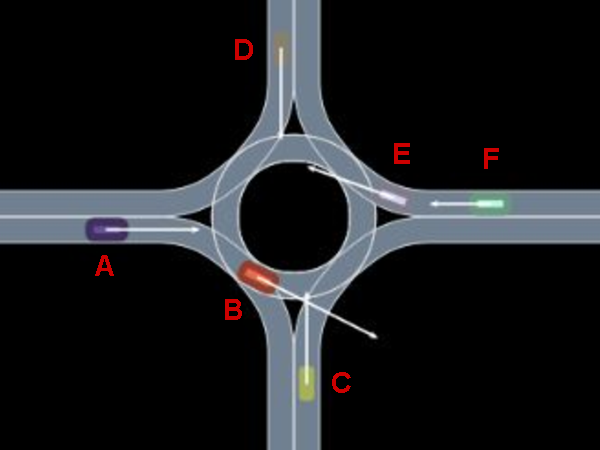
\includegraphics[width=0.8\linewidth]{figures/example_roundabout.pdf}
\caption{Vehicle F is on a collision course with E. C is on a collision course with B, but B is not on a collision course with C (because C should yield).}
\label{fig:collision}
\end{figure}

The collision course detection was eventually implemented with a special case for the roundabout.
\begin{lstlisting}[language=python, caption={Collision detection.}]
function on_collision_course(v1::Entity, v2::Entity)
	# check projection of velocity vectors
	vel1 = velg(v1.state)
	dx = (posg(v2.state) .- posg(v1.state))[1:2]
	projection = dot(dx, vel1)
	if projection > 5.0 && projection < 150
		return true
	end
	# SPECIAL CASE: if we are not in
	# the roundabout and the other vehicle is
	s1 = posf(v1.state).s
	s2 = posf(v2.state).s
	if (s1 < L|| s1 > 2L) &&
	   (s2 >= L && s2 <= 2L)
		return true
	end
	return false
end
\end{lstlisting}
\begin{figure}[h]
	\centering
	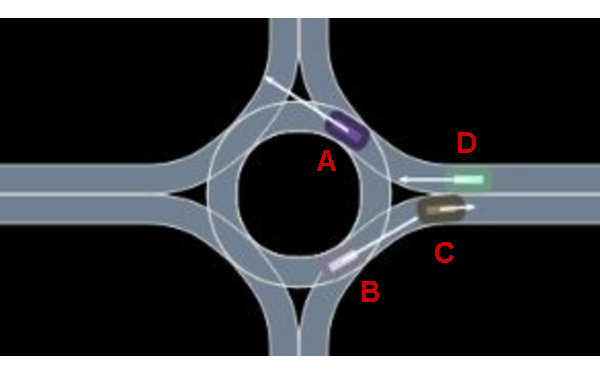
\includegraphics[width=0.8\linewidth]{figures/example_bug.pdf}
	\caption{Another potential challenge is excluding cases like D and C, where two vehicles are nearby but heading opposite directions in opposite lanes. D and C should not be on a collision course.}
	\label{fig:bug}
\end{figure}

\subsection*{Training}
We used 50 runs per epoch, checking the convergence condition $\|U_k-U_{k-1}\|_2 / \|U_k\|_2 <\epsilon$ at the end of each epoch. For all agents, $\epsilon$ was set to $5e^{-4}$. Between 75 and 100 epochs were necessary to converge.

The addition of rule-breaking drivers decreased the convergence rate (Figure \ref{fig:convergence}). However, all four agents were able to converge to a reasonably effective policy.


\begin{figure}[h!]
	\centering
	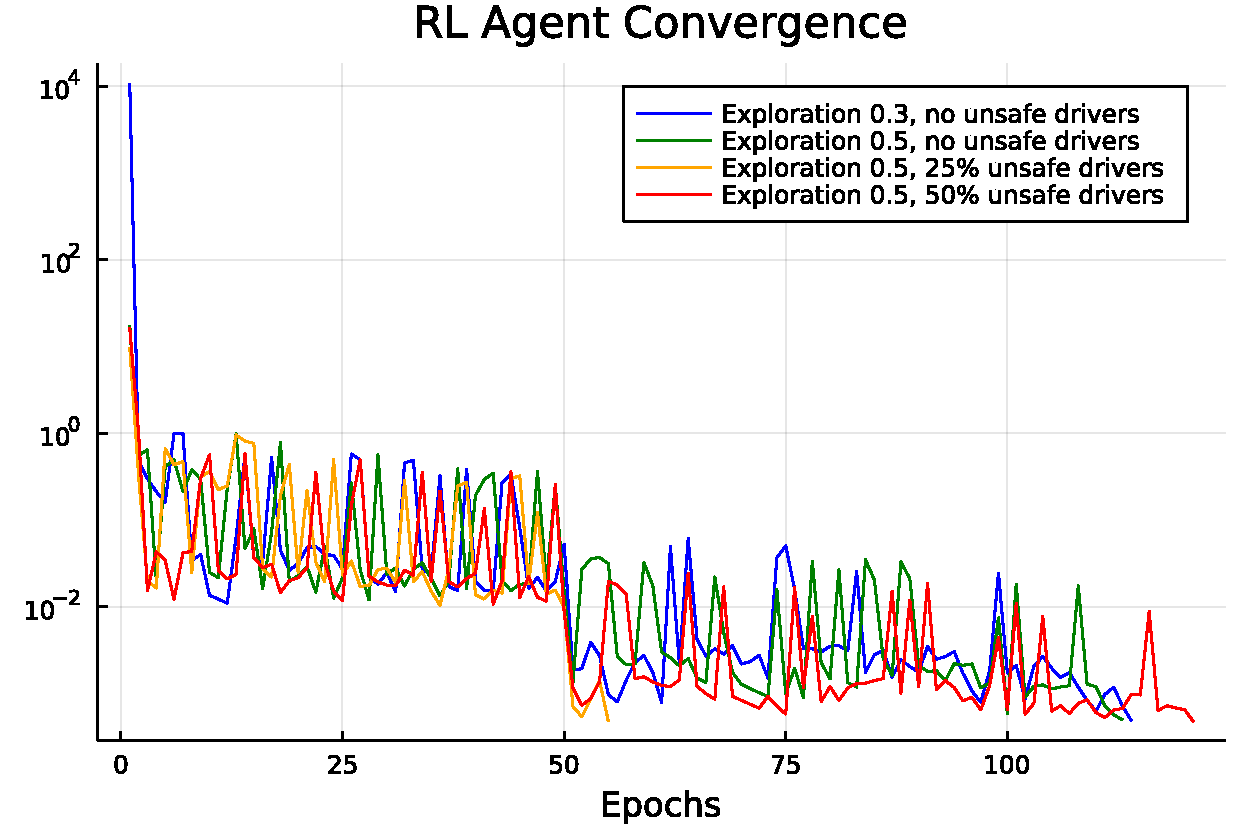
\includegraphics[width=1.0\linewidth]{figures/final_convergence.pdf}
	\caption{Convergence of four test cases for the final RL agent. The jump is where we re-started the training loop after pausing it to save a snapshot of the value function.}
	\label{fig:convergence}
\end{figure}

\section{Results}
 We trained four agents in total. To investigate the effect of the exploration rate $p$ (the probability of taking a random action), we trained one agent with $p=0.3$ and one with $p=0.5$, both in a simulation with no rule-breaking drivers. We found that the agent with the lower exploration rate performed noticeably worse, so we selected $p=0.5$ for the remaining agents.

The third agent was trained with $p=0.5$ and 20\% rule-breaking drivers in the roundabout (4 rule-following drivers and one rule-breaking).
The last agent was trained with $p=0.5$ and 40\% rule-breaking drivers (2 rule-breaking, 3 rule-following). This policy took the longest time to converge.

After training we ran multiple trials with each agent, sorting them into three categories based on outcome: completed (the agent successfully crossed the roundabout), passed (didn't cross, but didn't collide) and collisions.

\clearpage

With 4 vehicles in the roundabout, the rule-breaking and rule-following baselines performed best (Fig. \ref{fig:success_4cars}). The rule-breaking agent, in particular, never stopped to wait for another vehicle in the roundabout (Fig. \ref{fig:passes_4cars}). We weren't able to draw any conclusion about whether the agents trained with rule-breaking drivers were more cautious, resulting in fewer successful crossings and fewer collisions, from Figure \ref{fig:passes_4cars}.
\begin{figure}[h]
	\centering
	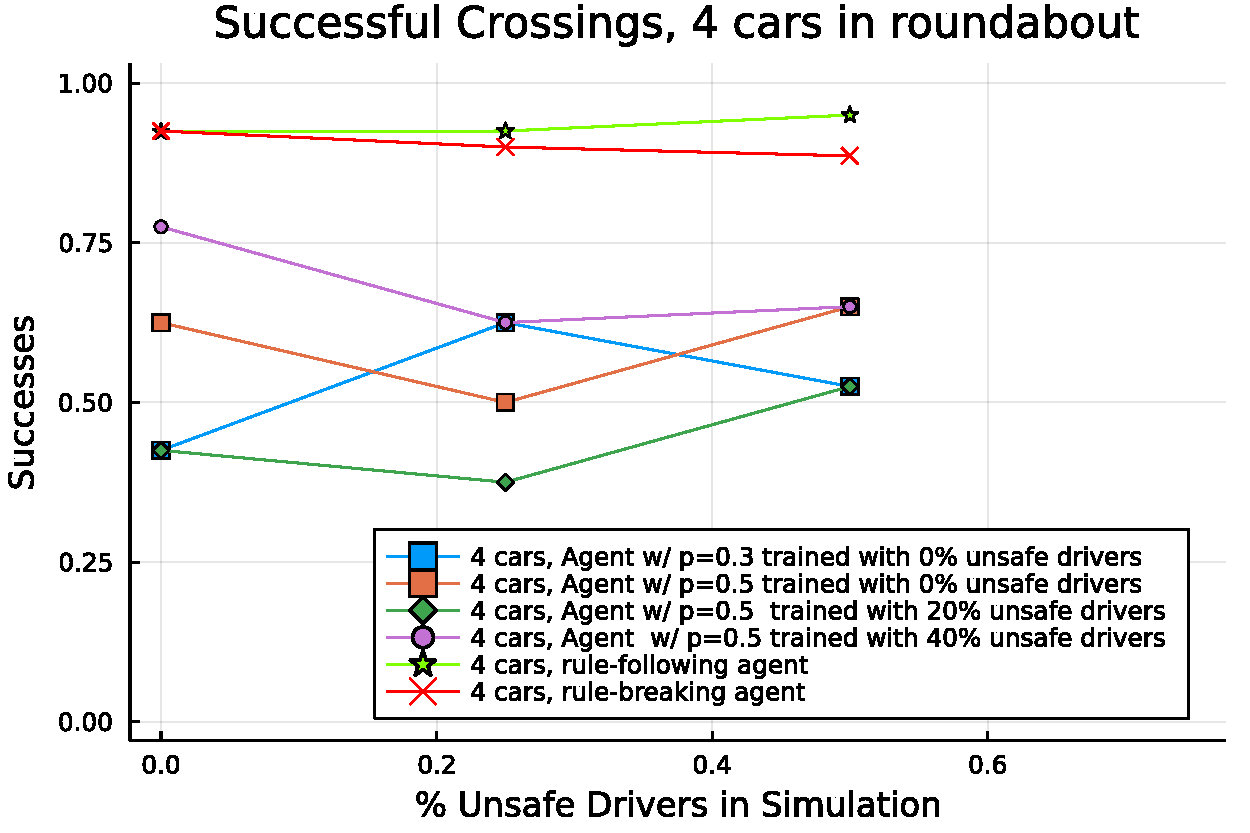
\includegraphics[width=0.9\linewidth]{figures/successes_3.pdf}
	\caption{Success rate with 4 cars in roundabout.}
	\label{fig:success_4cars}
\end{figure}
\begin{figure}[h]
	\centering
	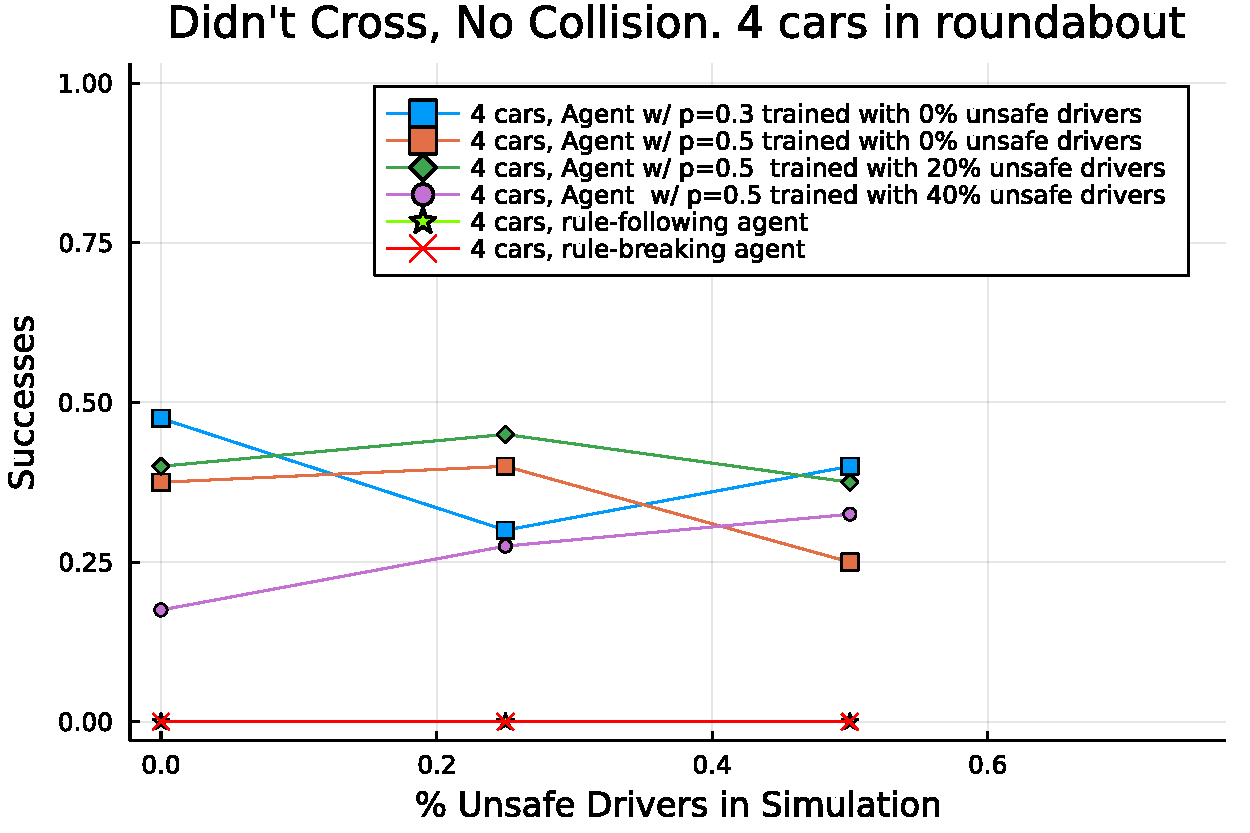
\includegraphics[width=0.9\linewidth]{figures/passes_3.pdf}
	\caption{Pass rate with 4 cars in roundabout.}
	\label{fig:passes_4cars}
\end{figure}
\begin{figure}[h]
	\centering
	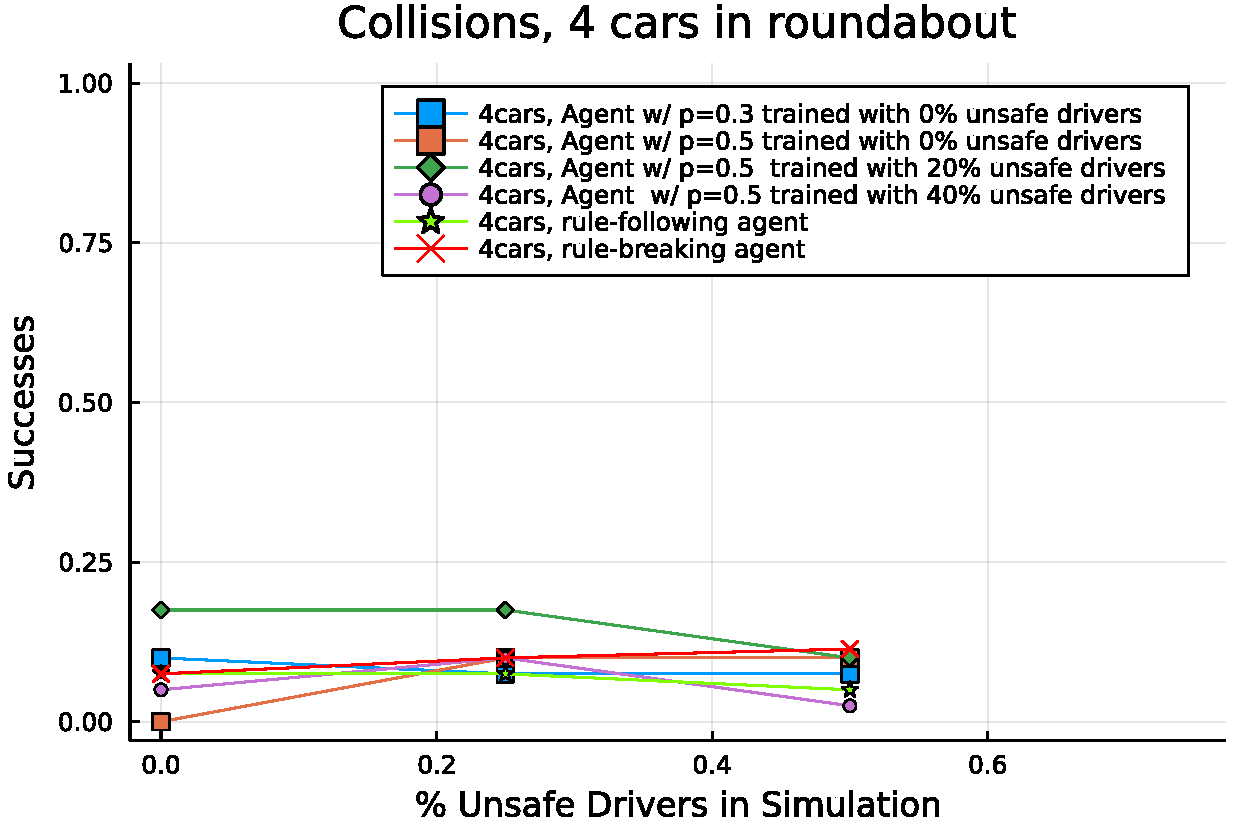
\includegraphics[width=0.9\linewidth]{figures/collisions_3.pdf}
	\caption{Collision rate with 4 cars in roundabout.}
	\label{fig:collisions_4cars}
\end{figure}

With 6 vehicles in the roundabout, performance was very poor with many collisions (Fig. \ref{fig:collisions_6cars}) and few successful attempts. All of the agents performed similarly poorly at crossing (Fig. \ref{fig:success_6cars} and \ref{fig:passes_6cars}), which suggests the rule-following and rule-breaking models are poorly implemented. Perhaps given better drivers to interact with, the RL agents would learn a more effective policy.

\begin{figure}[h]
	\centering
	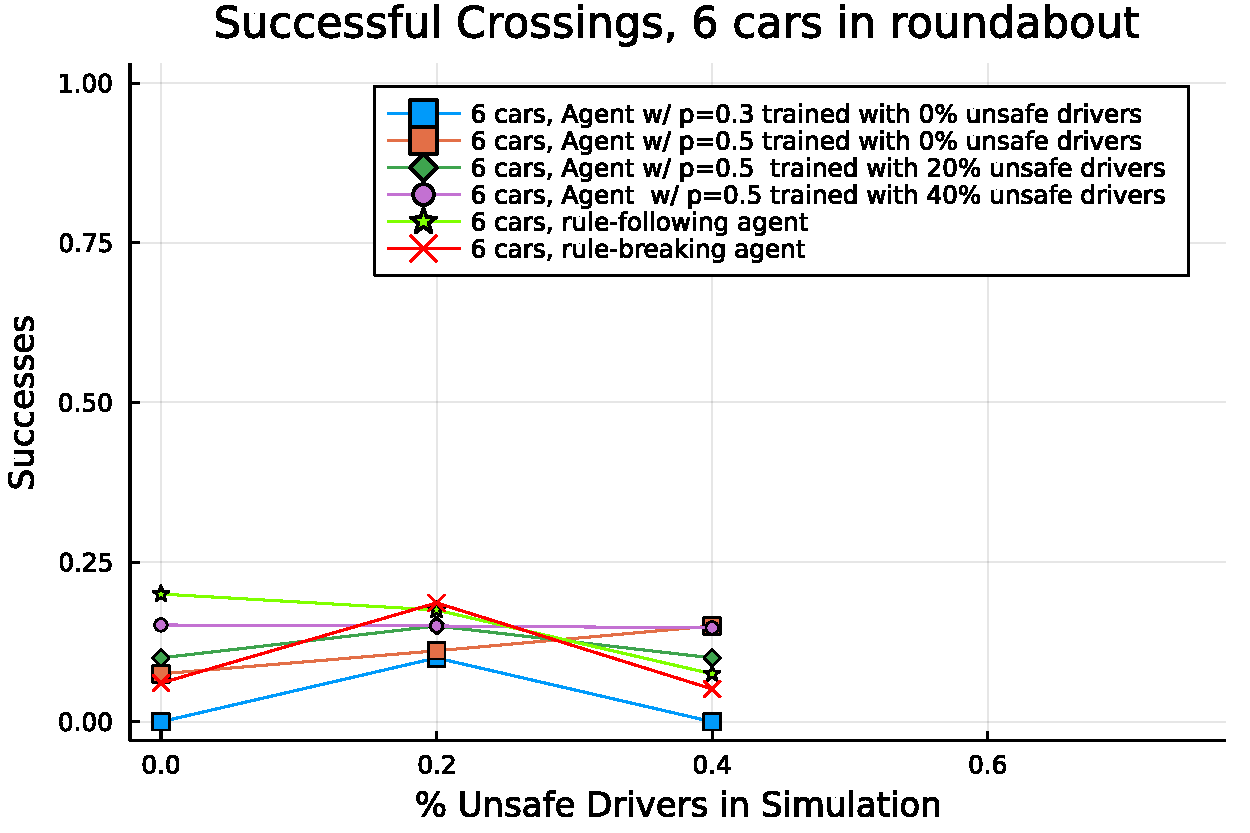
\includegraphics[width=0.9\linewidth]{figures/successes.pdf}
	\caption{Success rate with 6 cars in roundabout.}
	\label{fig:success_6cars}
\end{figure}
\begin{figure}[h]
	\centering
	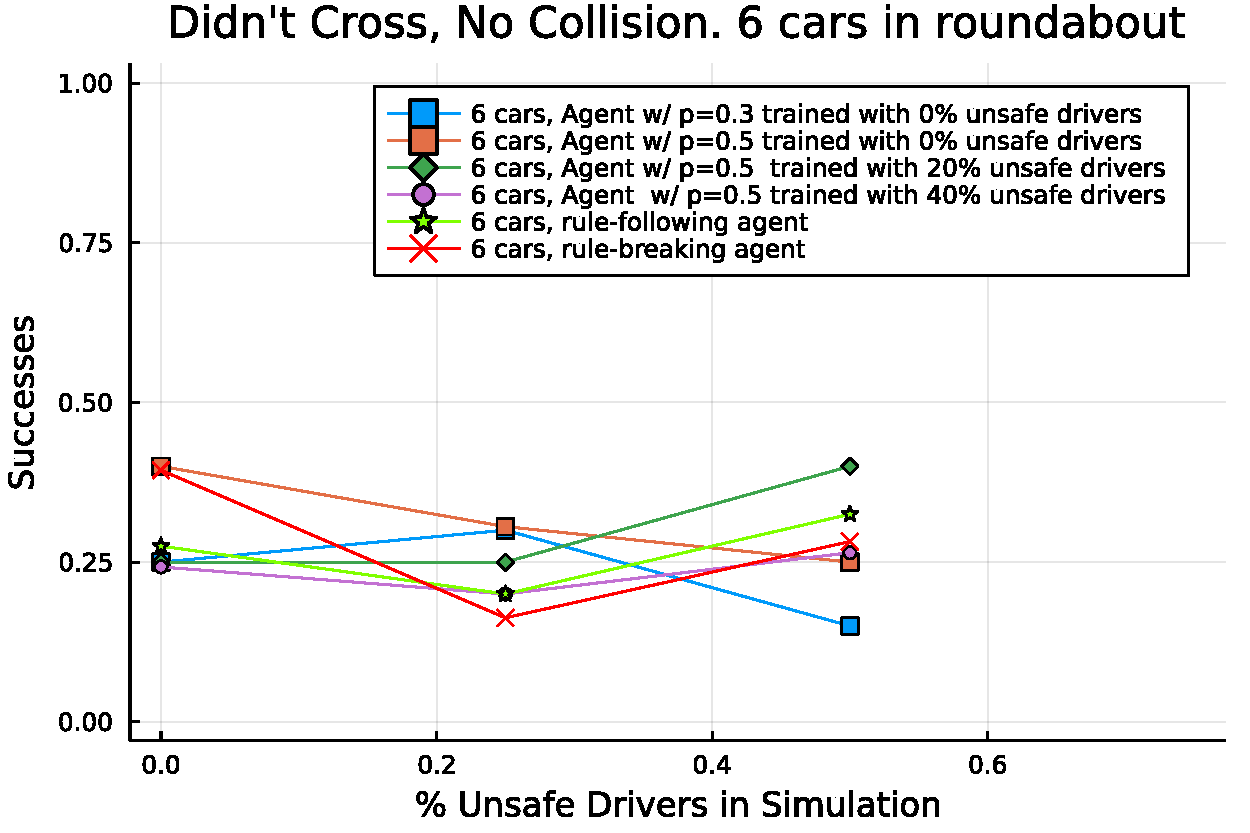
\includegraphics[width=0.9\linewidth]{figures/passes.pdf}
	\caption{Pass rate with 6 cars in roundabout.}
	\label{fig:passes_6cars}
\end{figure}
\begin{figure}[h]
	\centering
	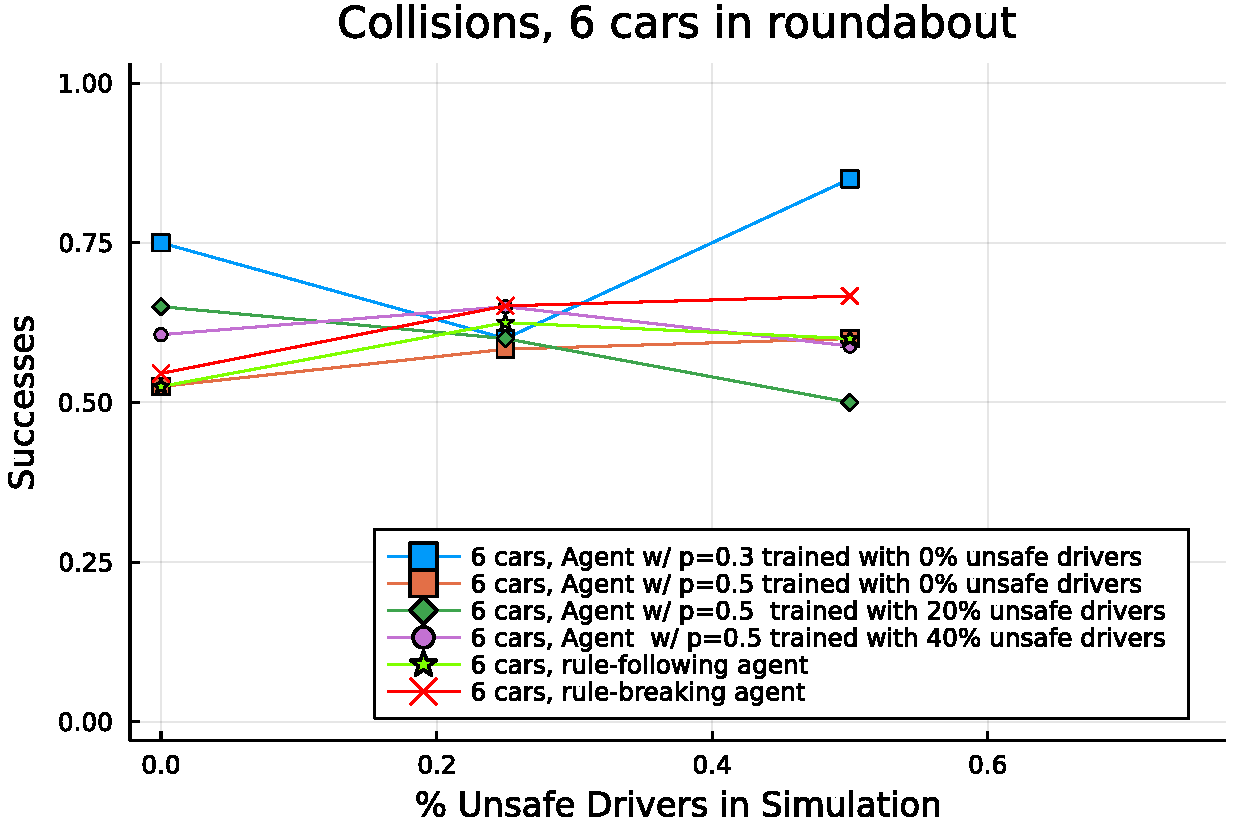
\includegraphics[width=0.9\linewidth]{figures/collisions.pdf}
	\caption{Collision rate with 6 cars in roundabout.}
	\label{fig:collisions_6cars}
\end{figure}

\clearpage

\begin{table}
	\begin{minipage}{\textwidth}
		\centering
		\begin{tabular}{|p{8em}|ccccc|}\hline
		Policy & Rule-breaking & \verb|exp03_unsafe_0| & \verb|exp05_unsafe_0| &  \verb|exp05_unsafe_20| &  \verb|exp05_unsafe_40| 
		\\\hline
		\% difference from rule-following & 8.1\% & 66.1\% & 67.7\% &67.1\% & 65.8\%
		\\
		\% with \verb|ACCEL| and \verb|DECEL| swapped vs rule-following & 6.7\% &
		26.7\% & 28.8\% &27.8 \% & 27.8\%
			\\\hline
		Policy & Rule-following & \verb|exp03_unsafe_0| & \verb|exp05_unsafe_0| &  \verb|exp05_unsafe_20| &  \verb|exp05_unsafe_40| 
		\\\hline
		\% difference from rule-breaking & 8.1\% & 66.9\% & 67.6\% &66.4\% &
		65.6\%
	\\
		\% with \verb|ACCEL| and \verb|DECEL| swapped vs rule-breaking & 6.7\% &
26.6\% & 28.1\% &26.7 \% & 27.1\%
\\\hline
		\end{tabular}
		\caption{Comparison of state-action pairs. The agents are named according to their exploration probability (\texttt{exp}) and the percentage of rule-breaking drivers present in their training (\texttt{unsafe}).}
		\label{tab:comparison}
	\end{minipage}
\end{table}

\section{Did RL actually work?} We would be remiss if we did not evaluate the RL agents skeptically, as RL has been accused of many misdeeds (including, on some problems, being no better than a random policy search \cite{mania2018simple}).
Since performance with many vehicles in the roundabout suffered from poor implementation of the rule-breaking and rule-following drivers, we compared the state-action maps of the RL agents against the rule-following and rule-breaking drivers themselves (Table \ref{tab:comparison}). Unfortunately all four of the RL agents differ on about two-thirds of the states, suggesting they do not converge to either agents' policy.


\section*{Conclusions}
Reinforcement learning was not very effective for this MDP. If we had additional time, we could implement other tactics to solve the roundabout navigation problem. For example, we could try formulating the problem as a large LP or using a better representation of the value function \cite{kochenderfer2022algorithmsch7}. Additionally, developing a better implementation for the rule-breaking and rule-following driver models would improve the simulation fidelity.

Despite these issues the Rl agents were able to navigate an un-crowded roundabout, even when rule-breaking drivers are present. We also resolved many problems with the state space and reward function design for the problem, so improvements to the remaining issues would likely yield much better performance.

Source code, data and figures for this paper can be accessed at \href{https://github.com/elsoroka/AA228-project-winter-2023}{https://github.com/elsoroka/AA228-project-winter-2023}.

\section*{Acknowledgments}
I would like to thank Prof. Kochenderfer and all of his TAs for being great this quarter, teaching a lot of interesting material and giving us the freedom to be creative with our final projects.

SISL developed the AutomotiveSimulator.jl package which provided a reliable base for RL training and simulations. All errors in software judgment are my own.

Finally, my original proposal was to use MDPs for modeling intersections. Credit for the switch to a more interesting topic goes to all of the sub-optimal drivers holding up traffic in Stanford's roundabouts.
\vspace{4em}\\
~
\\
\vspace{13em}

\bibliography{../bibliography}
\end{document}
